\documentclass{article}

\usepackage[utf8]{inputenc}
\usepackage[danish]{babel}
\usepackage{enumerate}
\usepackage{graphicx}
\usepackage{float}

\title{Slutrapport}
\author{Henrik Romby Mikkelsen og Jacob Scherffenberg-Møller}

\begin{document}

\maketitle
\tableofcontents
\pagebreak

\section{IT-projektets formål}

Projektets formål er at lette Skou Gruppens overblik, og kontrol med deres værktøj IT-Systemet vil kæde ansatte sammen med værktøj i form af udlån og aflevering. Yderligere vil systemet registrer værktøj, der er til reparation. Endvidere i forbindelse med vedligholdelse af værktøjet, vil der blive registreret datoer, et givet stykke tid før disse datoer, vil medarbejder i besiddelse af værktøj, der skal serviceres blive informeret i form af mail og evt. sms, så de kan komme tilbage til værktøjslageret og få et stykke værktøj, der er serviceret. 
Systemet vil i form af disse funktioner hjælpe virksomhedens ledelse, med at anskueliggøre om værktøj, der ikke længere er i virksomheden er bortkommet, eller om det er blevet kasseret, dette skulle gerne hjælpe ledelsen med at skære ned på omkostninger i forbindelse med bortkommet værktøj. 

\subsection{BATOFF}
\begin{figure}[htbp]
\begin{tabular}{ l p{8cm} }
\hline
Betingelser & Systemet skal kunne bruges af personer med begrænsede IT-kundskaber, hovedsageligt murere og tømrere, men også af kontoruddannede. \\
Anvendelsesområde & Firmaets ledelse -- eventuelt en lageransvarlig til administration af værktøj. Øvrigt ansatte til booking af værktøjer.  \\
Teknologi & Webbasseret, giver understøttelse af Mac OS, Windows, Linux og smartphone-styresystemer. \\
Objekter & Ansatte og værktøj. \\
Funktionalitet & Adminstration og service af værktøj.  \\
Filosofi & Adminstrativt IT-system. \\
\hline
\end{tabular}
\caption{BATOFF}
\end{figure}
\section{Kravspecifikation for IT-løsningen}
\begin{enumerate}
\item Ansatte skal på en nem og hurtig måde kunne booke of afleverer værktøj kvitteringer sendes, som email til en lageransvarlig og den givne medarbejder. Yderligere skal værktøj kunne overføres mellem to ansatte i firmaet. 

\item Ved oprettelse af nyt værktøj, skal der være mulighed for at knytte en kommentar til værktøjet, dette kan være et bilagsnummer, så man i forsikringsøjemed kan forefinde kvitteringer m.m.  

\item Værktøj skal serviceres inden for en given periode før dennes periodes udløb, skal systemet gøre opmærksom på at service er nødvendigt, hvis værktøjet er udlånt til en medarbejder notificeres denne om det forestående service. I det fald at værktøjet ikke er udlånt, skal den lageransvarlige notificeres. 

\item En samlet liste over alt firmaets værktøj skal kunne udskrives til brug ved optælling af værktøj. 

\item  Værktøj skal udover at kunne kaseres, noteres som værende bortkommet, dette dækker over flere hædelse, hvor værktøjet ikke længere er i firmaets varetægt. 

\item Alle objekter i systemet, skal tilknyttes en historik til adminstrativ brug, historikken skal vise et overskueligt antal af tidligere hændelser, hændelser der ryger ud af historikken for at gøre plads til nye, gemmes og kan efter behov tilgås. 

\item Der er blevet stillet ønske om mulighed for, at tilgå en mindre del af systemet fra smartphones i den mobile version er ønsket, at der kan lånes og afleveres værktøj. På denne måde har de ansatte en hurtig og simpel måde at få lånt værktøj, fremfor at skulle være på computer. 
\end{enumerate} 



\section{Teknisk platform}
\subsection{Udstyr}
Systemet er online så, der skal bruges en PC, MAC eller linux computer - Disse skal have en browser af nyere dato installeret. Endvidere vil der være mulighed for at tilgå systemet fra smarthphones. 
Endvidere er der behov for en server til hosting. 
Det skal være muligt for mere end en klient at tilgå systemet samtidig. 
\subsection{Basisprogrammel}
Systemet udvikles i det python baserede Django web framework, til systemet hører desuden en relationel database, på nuværende tidspunkt er denne baseret på SQLite, senere i udviklingen vil det være mere effektivt at skifte over til MYSql. Det kan diskuterres om det arbejds byrde mæssigt havde været mere effektivt at gå direkte igang med at bruge MYSql, men vores erfaring er at SQLite meget bekvemt i forbindelse med prototyping og test, derfor har vi valgt denne fremgangsmåde, og besluttet at MYSql så kan tages i brug på et senere tidpunkt, nå systemet skal opskaleres til større datamængder.  
\subsection{Systemgrænseflader} 
Systemet har ingen systemgrænseflader, det er en lukket database, som bruges af kontorpersonale og håndværkere. En mulig systemgrænseflade systemet kunne indeholde kunne være til et andet system, der kunne håndtere arbejdsplanlægning og regnskaber for virksomheden, dette er dog ikke en del af vort problemområde. 
\section{Arkitektur}
\subsection{Komponentarkitektur}

\subsection{Procesarkitektur}
Systemet skal ligge på en ekstern server, denne skal være i stand til at håndtere samtidige processer, da systemet kan tilgås at flere brugere sideløbende. Serverens evne til at håndtere samtidighed i systemet er essentiel, da de ansatte ellers ville kunne komme til at låne det samme stykke værktøj på samme tid, hvilket ikke er et ønskværdigt scenarie. 
Alle ansat har en personlig bruger i systemet, for at undgå problemer med samtidighed, hvor flere brugere brugte et enkelt login, og derved kunne komme til at "forstyrrer" hinandens arbejde.  
\section{Model- og funktionskomponent}

\section{Brugergrænsefladekomponent}
Brugergrænsefladen er under stadig udvikling, hvor der arbejdes med nogle forskelliger ideer, dette skyldes ikke, som sådan at den ene eller andet design har været dårligt, men at vi så vidt muligt vil skræddersy systemet til vores kunde, og give dem mulighed for at vælge, hvad de synes bedste dækker deres behov. Fælles for alle versioner er analogien til bibliotekker, en meget naturlig analogi i forbindelse med udlån og afleveringer af objekter.   
\subsection{1. Version}
I vores første version blev der arbejdet imod idealer, som kendes fra smartphones og tavlecomputere, hvor tydelige knapper er centralt i systemet, og man med få tryk kan navigerer til og fra alle dele af systemet. 

\begin{figure}[H]
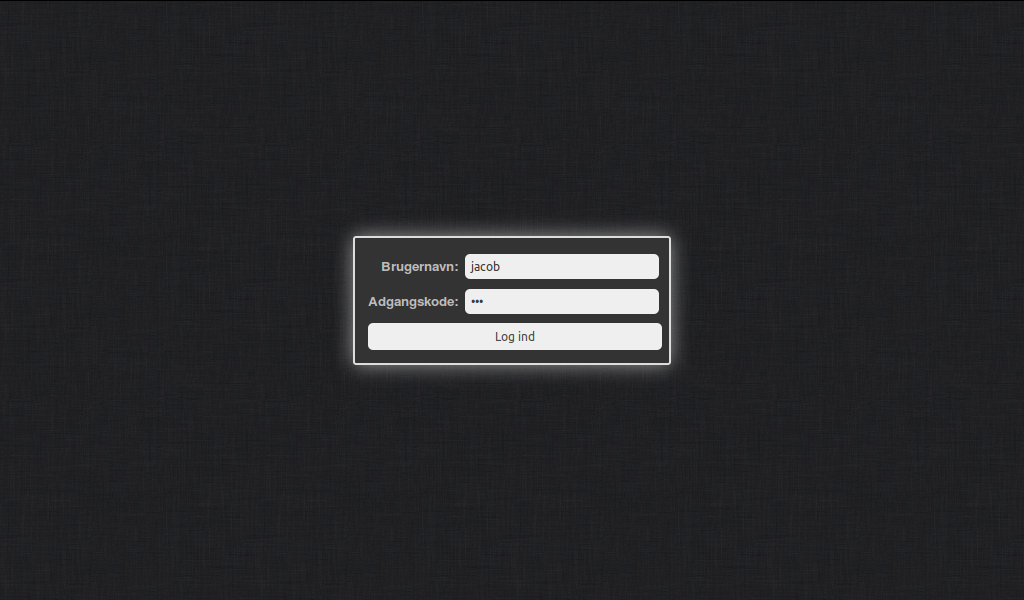
\includegraphics[scale=0.40]{./figures/loginpage.png}
\caption{Loginsiden byder brugeren velkommen til systemet med en meget almindelig login formular.}
\end{figure}


\begin{figure}[H]
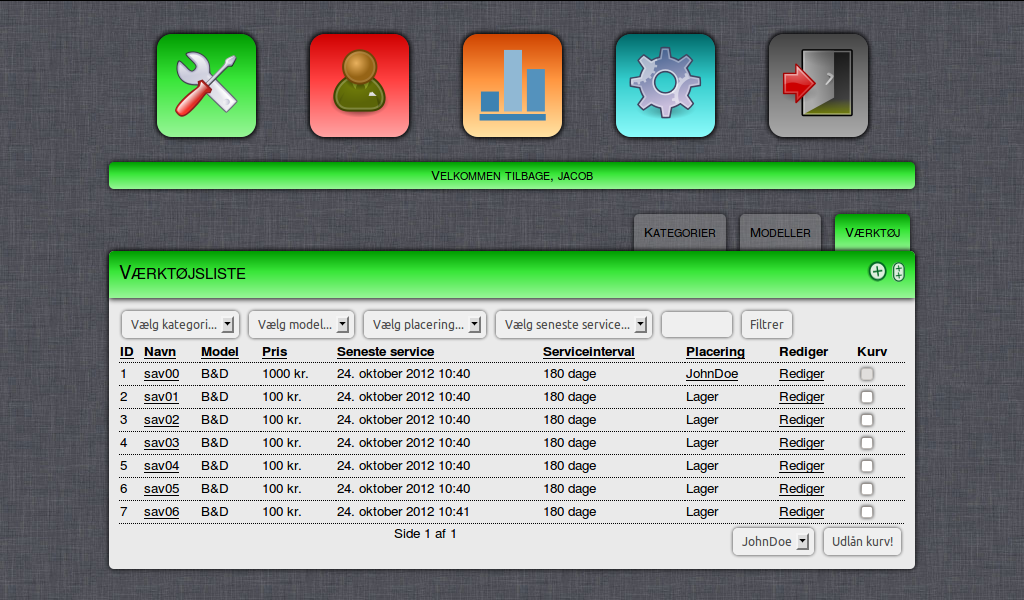
\includegraphics[scale=0.40]{./figures/tools.png}
\caption{Systemets værktøjsliste}
\end{figure}

Listen med værktøj er det første, der møder brugeren efter succesfuldt at være logget ind i systemet herfra kan værktøj lånes og afleveres, hvis en administrator er logget har denne yderligere muligheder med værktøjet. Der er kun få knapper i systemet, hvor størstedelen hele tiden er tilgængelige i toppen af billedet, disse kan udføre systemets hovedopgaver simpelt og med få klik. 

\begin{figure}[H]
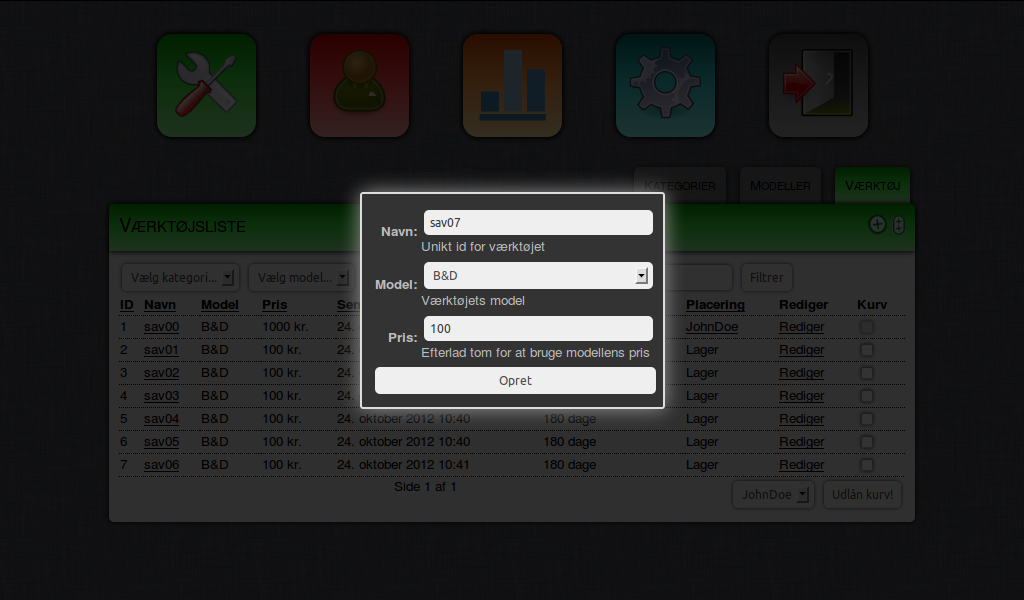
\includegraphics[scale=0.40]{./figures/createtool.png}
\caption{Formular til oprettelse af værktøj}
\end{figure}

Formularer som denne er indkorporeret, som en form for popup, fremfor at der åbnes et egentligt vindue. Der er en række formularer, som denne blandt andet også til oprettelse af nye ansatte. 

\begin{figure}[H]
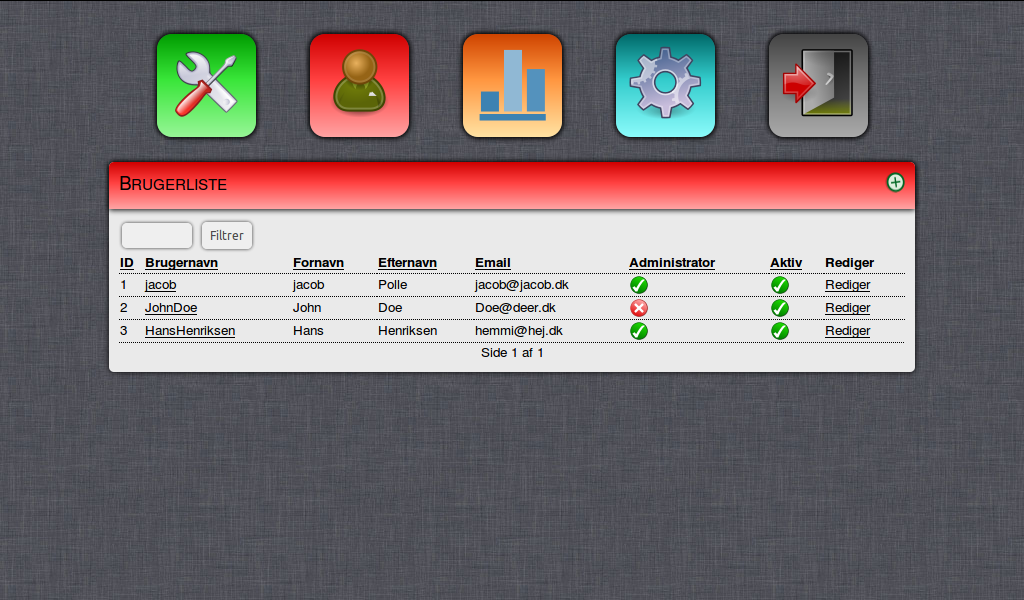
\includegraphics[scale=0.40]{./figures/Users.png}
\caption{Systemetets brugerliste. }
\end{figure}

Meget i tråd med værktøjslisten indeholder alle brugere, der er oprettet i systemet med tydelige afmærking af disses rettigheder, brugerlisten er kun tilgængelig for administartorer 

	
\subsection{2. Version prototype}
Efter at have revideret det første design, gik vi over til at arbejde med en analogi til det meget udbredte musik program Itunes. Itunes design sikrer en meget overskuelig og nem måde at se, hvilke kunstnere man har musik fra, hvilke af deres albummer man er i besiddelse af - herunder hvilke sange, der er på hvert album. Det er altid anbefalesesværdigt at arbejde med analogier, som denne da mange mennesker allerede kender Itunes, og derfor vil kunne genkende designet, dette sikrer at brugeren føler sig tryg i det nye system. 
Endvidere sikrer det at genbruge meget gennem testede ideer, at logikken i designet allerede er på plads, og at brugeren ikke skal til at sætte sig ind i et helt nyt system.
\section{Implementation af IT-løsningen}

\section{Evalueringer af IT-løsningen}
Systemet er blevet fremvist for kunden, hvor der blev evalueret på design og funktioner, der var ikke tale om en egentlig test af systemet, en sådan er planlagt nå designet er helt på plads, hvor systemet så vil blive taget i brug i en testperiode, på denne måde bliver systemet testet i så realistiske rammer, som muligt dette gør at den feedback vi kan få bliver mere specifik end ved en tænkt test. 
Ved den første evaluering blev der stille en række ønsker og krav til ændringer, herunder listes de 3 mest væsentlige. 
\begin{enumerate}
\item Den fulde værktøjsliste skal kunne udskrives, til brug ved status, og nå arbejdstilsynet kommer forbi. 

\item Værktøj skal ved oprettelse kunne tilknyttes en kommentar med bilagnumre, så kvitteringer m.v kan forefindes i forbindelse med forsikrings sager og lignende. 

\item Udover at værktøj kan kasseres, skal det også være muligt at markerer det, som bortkommet da det er væsentligt for administrationen at kunne se, hvor meget der smides ud kontra, hvor meget der forsvinder.
\end{enumerate}

Endvidere vil der være en evaluering af den 2. version af brugergrænsefladen nå denne er færdiggjort, dette vil være en uformel evaluering i stil med den måde første version blev evalueret på. 
Der er selvfølgelig visse fordele i at lave evalueringer mere formelle, f.eks. i form af en tænke højt test, hvor vi får set nogle af de kommende brugeres interageren med systemet. Dette er dog langt mere tidskrævende for både os og kunden, end den mere uformelle tilgang, og med planen om at lade systemet gennemløbe en test periode, hvor det bliver brugt i fuldt ud realistiske omgivelser fremfor en opsat test, hvor det er vores forestilling af systemets brug, der kommer til udtryk. 
Vi føler i denne forbindelse at de negative sider ved vores uformelle evalueringer, opvejes af den tid vi sparer på ikke at lave tænkte tests, men derimod får testet systemet med en realistisk workload og i de rigtige omgivelser.

\section{Projektsamarbejdet}

\section{IT-projektets formål}

\end{document}
